% !TEX root = mythesis.tex



%==============================================================================
\chapter{Jets and tagging}
\label{sec:jetsandtaggers}
%==============================================================================
The aim of this chapter is to provide a brief introduction about the jet formation and their reconstruction process using a jet reconstruction algorithm. Two different types of jet collections which are used in this thesis are discussed in detail. After the reconstruction of jets, they are identified by using the jet tagging algorithm. Two different types of jet tagging algorithms are described in the last section of this chapter. 
%==============================================================================
\section{Jets}
\label{sec:jetsandtaggers:jets}
%==============================================================================
Jets are extended particle showers originating from the hadronisation of a parton. Quarks and gluons are constrained to the confinement. Therefore, they hadronise into hadrons. These hadrons can be grouped into jets by a jet reconstruction algorithm. The jet reconstruction algorithm uses the energy deposited by the particle shower of charged and neutral particles in the calorimeter along with the information of tracks and vertices, to reconstruct a jet.

%==============================================================================
\subsection{Jet reconstruction algorithm}
\label{sec:jetsandtaggers:jets:algorithm}
%==============================================================================
The jet algorithm is used to reconstruct a four-vector from the hadronisation products of a parton that corresponds to the underlying parton four-vector. The jets that are considered in this thesis are reconstructed using the anti-$k_{\text{T}}$ jet algorithm.~\cite{antikt} 

The anti-$k_{\text{T}}$ algorithm is a sequential jet algorithm which takes four-vectors of individual particles as input and clusters them together until a certain threshold requirement is fulfilled. First, the distance between each object is calculated. This distance does not only depend on the geometry but also on the kinematic properties. The distance between two objects, $i$ and $j$ is given by the following expression:
\begin{equation}
	d_{ij} = \text{min}(p_{\text{T}i}^{-2} , p_{\text{T}j}^{-2})\frac{\Delta R_{ij}^{2}}{R} \,,
\end{equation}
where $p_{\text{T}}$ is the transverse momentum of each object and $\Delta R_{ij}$ is the angular distance calculated by $\Delta R_{ij} = \sqrt{\Delta \eta^{2}+\Delta\phi^{2}}$. R is called the \textit{radius parameter}, which defines a threshold value on a radius of the cone in which the objects should be considered.~\cite{thesis:tanja} For small-$R$ jets, it is set to be $R=0.4$, and for large-$R$ jets, it is set to be $R=1.0$. In this thesis, both small and large-$R$ jets have been used.

Then, the distance between the object and the beam is calculated by $d_{iB} = p_{\text{T}i}^{-2}$. If this distance is greater than $d_{ij}$, then the objects $i$ and $j$ are combined to form a jet. This process is performed till $d_{iB}<d_{ij}$, then the formed jet is considered as the final jet, and it is then removed from the list. This procedure is repeated until every object is taken out and all final jets have been obtained. An illustration of the behaviour of the anti-$k_{\text{T}}$ algorithm in $\eta-\phi$ plane is shown in Fig.\ \ref{fig:jetsandtaggers:jets:algorithm} in an event with few particles.~\cite{thesis:tanja}

\begin{figure}[hbt!]
	\centering
	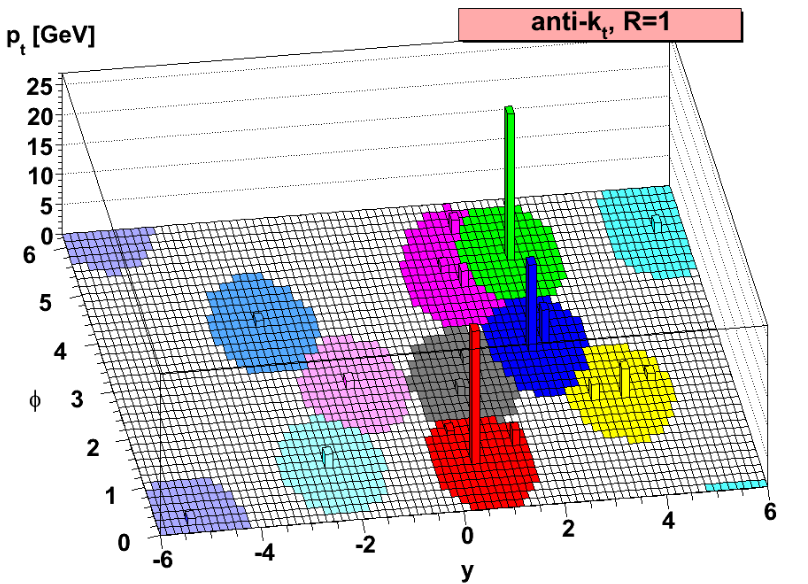
\includegraphics[width=0.6\linewidth]{jet_algorithm.png}
	\caption{A schematic showing the simulated event with several particles. Jets (in colour) are reconstructed using the anti-$k_{\text{T}}$ algorithm.~\cite{antikt}}
	\label{fig:jetsandtaggers:jets:algorithm}
\end{figure}

Jet energy has to be corrected before using the jets for event reconstruction because the detector response and the jet reconstruction algorithm are not perfect. The correction is performed such that the energy of the reconstructed jet corresponds to the energy of a jet reconstructed from the true stable particles in the detector. This procedure is called jet energy calibration.~\cite{jet_calibration}

Jets can be contaminated with partons from pile-up or underlying events, which can lead to a distortion of the jet four-momentum vector, which can cause not a good momentum resolution. This is usually common in large-$R$ jets because the probability to include hadrons that are not associated with the hard part of the interaction increases for a larger jet area. There are several methods to remove the contamination from the jets after reconstruction. One of the methods that are used in the ATLAS experiment is jet trimming.~\cite{jet_trimming} The jet trimming method uses the fact that the contribution from the pile-up or underlying event is usually softer than the contribution from the hard scattering.~\cite{thesis:ruth} 

Since a jet algorithm takes four-momenta as input, one can specify which information to use for the construction of the four-momenta. The ATLAS experiment uses calibrated calorimeter clusters to determine the four-momenta. Jets which are reconstructed based on calorimeter information are called calorimeter jets. Another method is to use the information of tracks along with the calorimeter information to determine the four-momenta for jet reconstruction. Jet reconstructed by using this method, is called particle flow jets. They both are discussed in detail in the next sections. The standard jet collection with a radius parameter of $R=0.4$ used by the ATLAS collaboration is a calorimeter jet.~\cite{thesis:ruth}

%==============================================================================
\subsection{Topo-cluster jets}
\label{sec:jetsandtaggers:jets:topo}
%==============================================================================
A calorimeter is divided into small units called cells. The signal produced in these cells corresponds to the input to a clustering algorithm to form a cluster. The topo-cluster formation algorithm starts from a seed cell, whose signal-to-noise (S/N) ratio is above a threshold value. Here, noise refers to an average expected noise in that cell. Another threshold value is set in order to include the neighbouring cells to the seed to form a protocluster. This process takes place iteratively where the S/N of all the neighbouring cells of the protocluster is evaluated. If it passes the threshold, it is merged to the protocluster. Finally, all calorimeter cells neighbouring the formed protocluster are added, which forms the topo-cluster. The topo-cluster algorithm efficiently suppresses the calorimeter noise. All the threshold are optimised for the clustering algorithm.~\cite{thesis:tanja}

The topo-cluster algorithm also includes a splitting step to optimise the separation of showers from other close-by particles. In a topo-cluster, all cells are searched for a local maxima (maximum energy) with a threshold of \SI{500}{\mega\electronvolt}. The local maxima are then used as seeds for a new iteration of topological clustering, which splits the original cluster into more topo-clusters. The jet finding algorithm considers only topo-clusters with positive energy. Fig.\ \ref{fig:jetsandtaggers:jets:topo} shows an example of the formation of topological clusters where each small unit represents a calorimeter cell, and its colour represents the amount of energy deposited in it. These cells are grouped into topo-clusters shown by black lines that represent the borders of the topo-clusters.~\cite{thesis:tanja} 

\begin{figure}[hbt!]
	\centering
	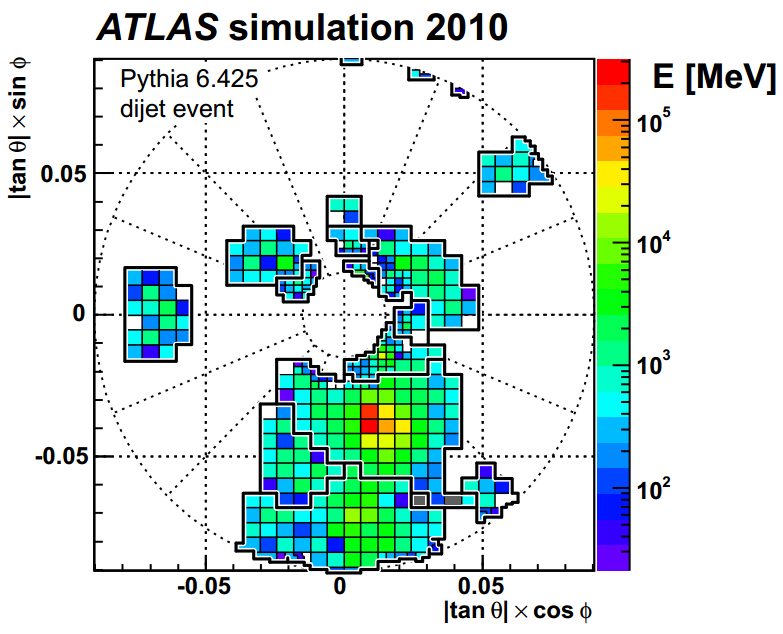
\includegraphics[width=0.6\linewidth]{topo.png}
	\caption{A schematic showing an example of the formation of topo-cluster using a clustering algorithm.~\cite{topocluster}}
	\label{fig:jetsandtaggers:jets:topo}
\end{figure}

After the clusters are formed by using the topo-cluster algorithm, anti-$k_{\text{T}}$ algorithm is used to reconstruct the topo-cluster jets. Two different jet calibrations are used in this thesis.  Small-$R$ jets are calibrated using the electromagnetic (EM) scheme, whereas large-$R$ jets are calibrated using the local cluster weighting (LCW) scheme. The main difference between the LCW and EM calibration schemes is that the LCW calibration classifies clusters as either being electromagnetic or hadronic in origin, whereas the EM calibration does not. Then, based on this classification, the LCW applies an energy correction that is dependent on the type of particle which created the calorimeter deposit.

%==============================================================================
\subsection{Particle flow jets}
\label{sec:jetsandtaggers:jets:pflow}
%==============================================================================
Particle flow (PFlow) jet reconstruction is introduced to take full advantage of all the particle sub-detectors to improve the energy resolution of reconstructed physics objects. The primary motivation for using particle flow is that at low energy, the tracking detectors provide a better \pt resolution for charged particles than the calorimeters. The \pt resolution ($\sigma_{\pt}$) of a charged particle in the ATLAS tracking detectors can be expressed as:~\cite{atlas}

\begin{equation}
	\frac{\sigma_{\pt}}{\pt} = 0.05\%\pt \oplus 1\% \,,
\end{equation}
where \pt is in units of \si{\giga\electronvolt}.

Fig.\ \ref{fig:jetsandtaggers:jets:pflow1} shows the \pt resolution as a function of \pt for charged particles in the EM and hadronic calorimeters compared to the tracking \pt resolution. It can be seen in this figure that at low \pt, the \pt resolution of particles is better in the tracker than the calorimeters. Therefore, if the \pt measurement from the tracker is used instead of the calorimeter deposits for low-\pt charged particles, there should be an improved \pt resolution for those charged particles.

\begin{figure}[hbt!]
	\centering
	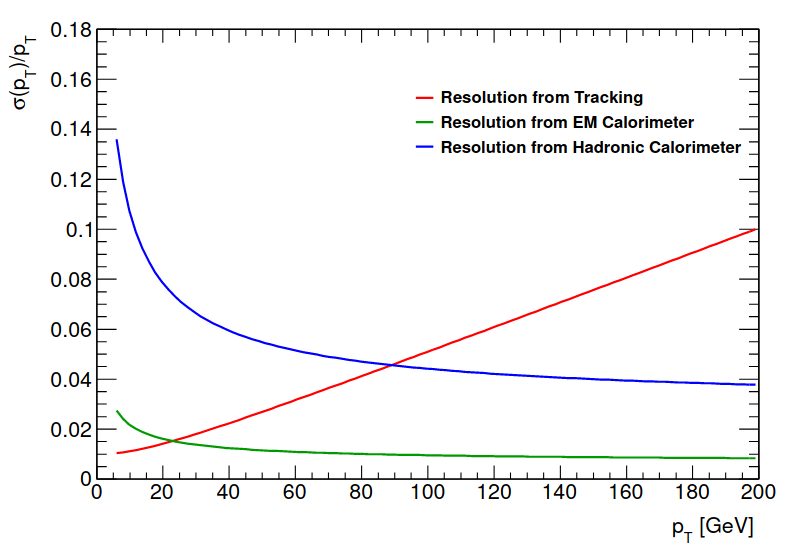
\includegraphics[width=0.6\linewidth]{pflow1.png}
	\caption{A plot showing the \pt resolution response as a function of \pt for the charged particles. It shows the response for EM and hadronic calorimeter along with the tracking detector.~\cite{atlas}}
	\label{fig:jetsandtaggers:jets:pflow1}
\end{figure}

At the LHC, particle flow has been used by the CMS experiment. In many searches in the ATLAS experiment, particle flow jets are used especially in SUSY and BSM searches, where it is potential to improve the jet energy resolution.

The particle flow algorithm is divided into four different stages, which are described in detail below:

\begin{itemize}
	\item \textbf{Track-cluster matching:} the tracks reconstructed from the hits in the ATLAS inner detector are extrapolated to the calorimeter. This provides the impact parameter coordinates of the extrapolated tracks to different layers of the calorimeters. These extrapolated impact parameter coordinates are then used to find the topo-cluster (described in previous section) that are closest to the extrapolated track. If no track is matched to the topo-cluster, it remained unmodified, and the measurements from the calorimeters are used. The cluster made from the neutral particle is treated as a neutral cluster by the particle flow algorithm. However, if tracks are matched to the cluster, then the cluster continued to the second step, which is charged shower subtraction process.~\cite{pflow}
	
	\item \textbf{Charged shower subtraction:} it is the removal of energy from calorimeter cell deposits from the clusters with associated tracks to avoid any double-counting of energy already deposited by the charged particles in the calorimeters. The amount of energy removed is determined by measuring the calorimeter response ($E/p$). It is defined as the ratio of the energy of a cluster in the calorimeter to the momentum of an associated track. $E/p$ varies depending on the region of the calorimeter and the energy of the incident particle. The energy is subtracted from calorimeter cells in the topo-cluster until the total amount of energy subtracted from the cluster is consistent with the fraction from the $E/p$ distribution.~\cite{pflow} 
	
	\item \textbf{Cluster annihilation:} it includes the removal of calorimeter clusters with associated tracks. If the remaining energy after subtraction is zero, the cluster is removed.
	
	\item \textbf{Neutral particle calibration:} the particle flow algorithm is performed before the calibration is performed on topo-clusters. So the energy deposits in the calorimeter are at the EM scale. After the charged shower subtraction process, only neutral deposits remained in the calorimeter. Therefore, these clusters should be fully calibrated to the appropriate energy scale. Otherwise, jets formed with the remaining topo-clusters would not be properly calibrated.
	
\end{itemize}


%==============================================================================
\section{Tagging}
\label{sec:jetsandtaggers:taggers}
%==============================================================================
After the jets are reconstructed, tagging is performed on the jets. Tagging is an identification of the jets originating from the decay of a particle. In this, working point (WP) describes the efficiency of tagging, for example, if tagging is performed at 70\% WP that means 70\% of all the jets which are originating from the decay of that particle are getting tagged by the jet tagging algorithm. This section summarises the two different types of tagging used in this thesis which include different jet tagging algorithm or taggers.

%==============================================================================
\subsection{$W$-tagging}
\label{sec:jetsandtaggers:taggers:w}
%==============================================================================
$W$-tagging is an identification of a jet originating from the decay of $W$ boson. It is implemented on large-$R$ jets because all-hadronic decay products of $W$ boson are boosted and can be reconstructed within a single large-$R$ jet. It is performed by a $W$-tagging algorithm which uses the jet substructure information to perform $W$-tagging. The two $W$-tagging algorithms which are based on the jet substructure variables and are used to perform $W$-tagging in this thesis are discussed in detail below:~\cite{wtagger}

%==============================================================================
\subsubsection{Two-variable tagger}
\label{sec:jetsandtaggers:taggers:twovariable}
%==============================================================================
The two-variable tagger is used for $W$ tagging of anti-$k_{\text{T}}$ large-$R$ jets of $R=1.0$.~\cite{wtagger} It is locally calibrated for two working points 50\% and 80\% of flat signal efficiency by using the topo-clusters trimmed jets as inputs. The tagger uses two substructure variables to tag $W$ jets: the combined jet mass $m^{\text{comb}}$ and $D_{2}$ variable. $D_{2}$ is a ratio of energy-correlation functions, approximately given by:~\cite{d2}

\begin{equation}
	D_{2} \approx \frac{p_{2}}{p^{2}} \text{ max}(\theta^{2},\theta_{2}^{2}) \,,
\end{equation}
where $p$ is denoted as the momentum of emission with which the jet mass is dominated and $p_{2}$ is denoted as the sum of the momentum of all the other emissions, and $\theta$ and $\theta_{2}$ are the emission angles of the two momenta respectively.

The tagger is optimised with respect to signal jets that are matched to a truth $W$ boson and that have a truth groomed jet mass of $\SI{50}{\giga\electronvolt} < m^{\text{comb}} < \SI{100}{\giga\electronvolt}$ for $W$-tagging. The tagger is optimised using the flat \pt signal sample of $W'\rightarrow WZ\rightarrow qqqq$ against QCD multijet events in MC16d.~\cite{wtagger}

Fig.\ \ref{fig:jetsandtaggers:taggers:twovariable} shows the resulting background rejections as a function of jet \pt for a selection of the most powerful two-variable combinations. Based on this plot, in the case of $W$-tagging, the combination of $m^{\text{comb}}$ and $D_{2}$ is most powerful in the kinematic range of interest and is taken as the baseline pairing for $W$-tagging. However, at higher jet \pt, where the power of $D_{2}$ decreases, it retains constant discrimination power. $W$-tagging for topo-cluster jets calibrated to LCW scheme are only supported up to \SI{2.5}{\tera\electronvolt} due to the degradation of the combined jet mass definition.

\begin{figure}[hbt!]
	\centering
	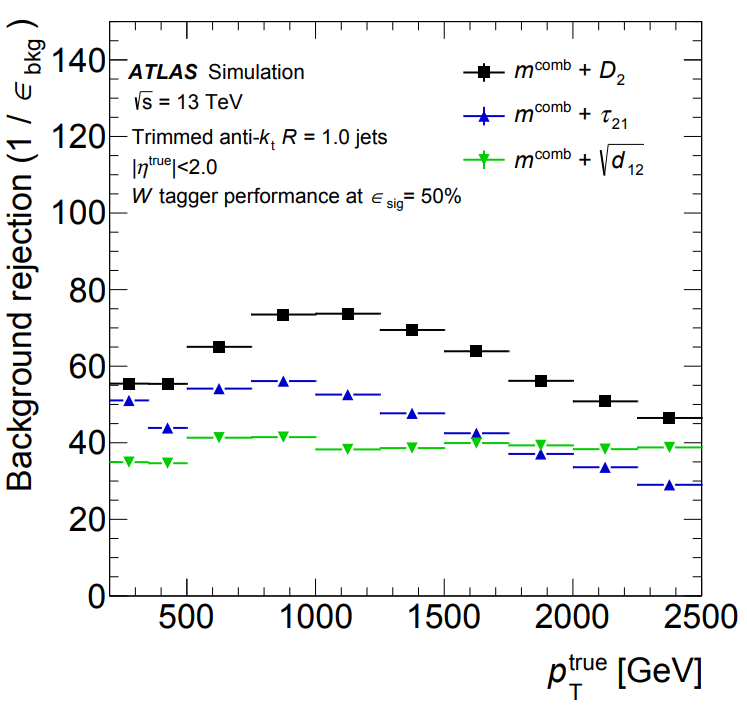
\includegraphics[width=0.5\linewidth]{two-variable_sig1.png}
	\caption{A plot shows the background rejection of $W$-tagging as a function of \pt at a fixed 50\% signal efficiency working point. It shows the response for three different combinations of jet substructure variables.~\cite{wtagging}}
	\label{fig:jetsandtaggers:taggers:twovariable}
\end{figure}

%==============================================================================
\subsubsection{Three-variable tagger}
\label{sec:jetsandtaggers:taggers:threevariable}
%==============================================================================
The three-variable tagger is also used for $W$-tagging of large-$R$ jets which is locally calibrated on two working points 50\% and 80\% of flat signal efficiency. The tagger uses three substructure variables to perform $W$-tagging: the combined jet mass $m^{\text{comb}}$, $D_{2}$ variable and Ntrk. Ntrk is a number of ghost tracks associated with the ungroomed jet of $\pt>\SI{0.5}{\giga\electronvolt}$. The tagger is optimised using the flat \pt signal sample of $W'\rightarrow WZ\rightarrow qqqq$ against QCD multijet events in MC16d.~\cite{wtagger}

Fig.\ \ref{fig:jetsandtaggers:taggers:threevariable} shows background rejection of the three-variable tagger as a function of jet \pt. It shows the response at two signal efficiency working points, i.e.\ 50\% and 80\%. One can compare the background rejection response of three-variable tagger with the two-variable tagger shown in Fig.\ \ref{fig:jetsandtaggers:taggers:twovariable} and notice that three-variable tagger has better rejection power at 50\% working point. These taggers show the best results at around \SI{1}{\tera\electronvolt} and then rejection power gradually decreases at higher \pt. At 80\% working point, the rejection power decreases, as expected, since it has lower selection criteria as compared to 50\% working point.

\begin{figure}[hbt!]
	\centering
	\begin{subfigure}{.45\textwidth}
		\centering
		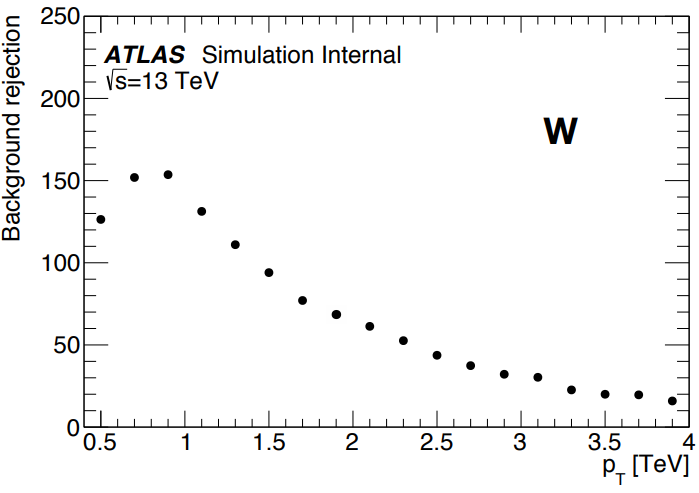
\includegraphics[width=\linewidth,height=\textheight,keepaspectratio]{three-variable_50.png}
		\caption{}
		\label{fig:jetsandtaggers:taggers:threevariable:50}
	\end{subfigure}\hspace{0.3cm}
	\begin{subfigure}{.45\textwidth}
		\centering
		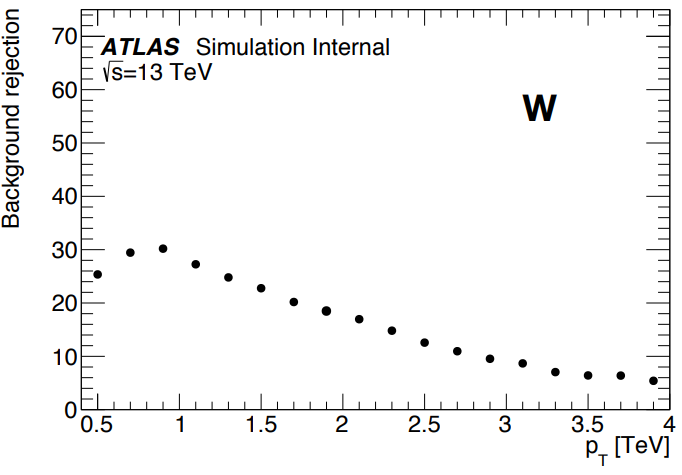
\includegraphics[width=\linewidth,height=\textheight,keepaspectratio]{three-variable_80.png}
		\caption{}
		\label{fig:jetsandtaggers:taggers:threevariable:80}
	\end{subfigure}
	\caption{The plots are showing the background rejection of three-variable tagger at a fixed (a) 50\% and (b) 80\% signal efficiency working point as a function of jet \pt.~\cite{wtagger}}
	\label{fig:jetsandtaggers:taggers:threevariable}
\end{figure}

Fig.\ \ref{fig:jetsandtaggers:taggers:threevariable:signal} shows the $W$-tagging efficiency of the three-variable tagger as a function of \pt along with the individual responses of all the three jet substructure variables. One can see that the mass efficiency cut started dropping after \SI{1.5}{\tera\electronvolt} whereas the other efficiencies increase at high \pt. The efficiency of $D_{2}$ variable has a higher $W$-tagging efficiency among the other two substructure variable. That is why it is the main input of these two $W$-tagging algorithms. 

\begin{figure}[hbt!]
	\centering
	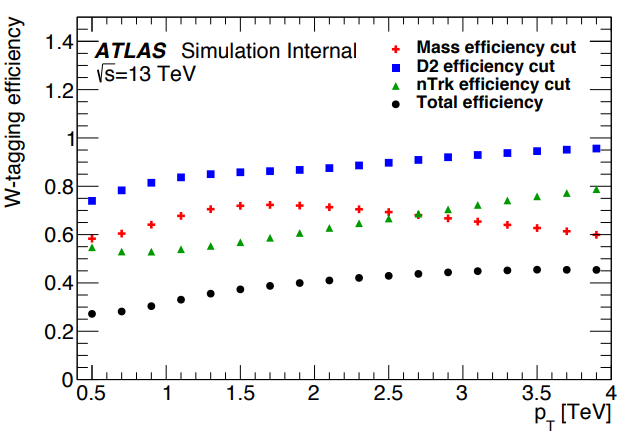
\includegraphics[width=0.5\linewidth]{three-variable_wtagging_efficiency.png}
	\caption{A plot is showing the $W$-tagging efficiency of three-variable tagger as a function of jet \pt. It also shows an individual response of all the three jet substructure variables.~\cite{wtagger}}
	\label{fig:jetsandtaggers:taggers:threevariable:signal}
\end{figure}



%------------------------------------------------------------------------------
\subsection{$b$-tagging}%
\label{sec:analysisstrategy:physicsobjets:bjets}
%------------------------------------------------------------------------------
$b$-tagging is an identification of jets originating from the decay of $b$-quark. It is one of the important selection criteria for this analysis. Jets originating from bottom quarks (called $b$-jets) are identified by reconstructing secondary and tertiary vertices from the tracks associated with the jets. The idea behind this is when a $b$-quark is produced, it hadronises and produce $B$-hadrons. They have an interesting property of a long lifetime. That means they can travel a measurable distance before they further decay. This distance is in order of few millimetres. So, if there is a secondary vertex (where $B$-hadron decays) which is displaced from the primary vertex (point of collision) in a jet, the jet can be tagged as $b$-jet. Moreover, due to the large mass of $B$-hadron, the decay products of $B$-hadron may have large \pt and large opening angle.~\cite{thomson}

The $b$-tagging algorithm used in this analysis is a multivariate algorithm called MV2c10, where training is performed on signal $b$-jets against a mixture background of about $90\%$ light-flavoured jets and $10\%$ $c$-jets. There are several working points which are provided for $b$-tagging. They are defined by a single cut on the MV2c10 output so that a particular $b$-jet efficiency is satisfied.~\cite{thesis:rui} Table \ref{table:analysisstrategy:physicsobjets:bjets} summarises the efficiencies for different working points. It also shows the cut value on the output for each of these working points. The rejection of $c$-jets and light-flavoured jets are also shown in the table. Rejection is calculated such that one out of this number of jets is misidentified as $b$-jet. 

\begin{table}[hbt!]
	\centering
	\begin{tabular}{c | c | c | c} 
		\toprule
		Working point & Cut value on output & $c$-jet rejection & Light-jet rejection \\
		\midrule
		60\% & 0.9349 & \num{34} & \num{1538} \\
		70\% & 0.8244 & \num{12} & \num{381} \\
		77\% & 0.6459 & \num{6} & \num{134} \\
		85\% & 0.1758 & \num{3.1} & \num{33} \\
		\bottomrule
	\end{tabular}
	\caption{Efficiency and cut value on output for each of the working points of the MV2c10 algorithm. Rejection of $c$-jets and light-flavoured jets are also shown. The values are estimated using a simulated $t\bar{t}$ sample.~\cite{thesis:rui}}
	\label{table:analysisstrategy:physicsobjets:bjets}
\end{table}

In this analysis, $70\%$ working point is chosen to balance $b$-tagging efficiency and rejection power. It requires the MV2c10 score to be higher than \num{0.8244}, which corresponds to a rejection factor of $c$-jets and light-flavoured jets to be 12 and 381 respectively. The $b$-tagging is performed on small-$R$ jets and the small-$R$ jets satisfying these criteria are referred to as $b$-jets. 



%%% Local Variables: 
%%% mode: latex
%%% TeX-master: "mythesis"
%%% End: 